%%%%%%%%%%%%%%%%%%%%%%%%%%%%%%%%%%%%%%%%%%%%%%%%%%%%%%%%%%%%%%%%%%%%%%%%%%%%%%%%%%%%%%%%%%%%%%%%%%%%%%%%%%%%%%%%%%%%%%%%%%%%%%%%%%%%%%%%%%%%%%%%%%%%%%%%%%%
% This is just an example/guide for you to refer to when submitting manuscripts to Frontiers, it is not mandatory to use Frontiers .cls files nor frontiers.tex  %
% This will only generate the Manuscript, the final article will be typeset by Frontiers after acceptance.   
%                                              %
%                                                                                                                                                         %
% When submitting your files, remember to upload this *tex file, the pdf generated with it, the *bib file (if bibliography is not within the *tex) and all the figures.
%%%%%%%%%%%%%%%%%%%%%%%%%%%%%%%%%%%%%%%%%%%%%%%%%%%%%%%%%%%%%%%%%%%%%%%%%%%%%%%%%%%%%%%%%%%%%%%%%%%%%%%%%%%%%%%%%%%%%%%%%%%%%%%%%%%%%%%%%%%%%%%%%%%%%%%%%%%

%%% Version 3.4 Generated 2018/06/15 %%%
%%% You will need to have the following packages installed: datetime, fmtcount, etoolbox, fcprefix, which are normally inlcuded in WinEdt. %%%
%%% In http://www.ctan.org/ you can find the packages and how to install them, if necessary. %%%
%%%  NB logo1.jpg is required in the path in order to correctly compile front page header %%%

\documentclass[utf8]{frontiersSCNS} % for Science, Engineering and Humanities and Social Sciences articles
%\documentclass[utf8]{frontiersHLTH} % for Health articles
%\documentclass[utf8]{frontiersFPHY} % for Physics and Applied Mathematics and Statistics articles

%\setcitestyle{square} % for Physics and Applied Mathematics and Statistics articles
\usepackage{url,hyperref,lineno,microtype,subcaption}
\usepackage[onehalfspacing]{setspace}

\linenumbers


% Leave a blank line between paragraphs instead of using \\


\def\keyFont{\fontsize{8}{11}\helveticabold }
\def\firstAuthorLast{Sample {et~al.}} %use et al only if is more than 1 author
\def\Authors{Philippe Massicotte\,$^{1,*}$, Tim Perry\,$^{2}$ and Emmanuel Devred\,$^{2}$}
% Affiliations should be keyed to the author's name with superscript numbers and be listed as follows: Laboratory, Institute, Department, Organization, City, State abbreviation (USA, Canada, Australia), and Country (without detailed address information such as city zip codes or street names).
% If one of the authors has a change of address, list the new address below the correspondence details using a superscript symbol and use the same symbol to indicate the author in the author list.
\def\Address{$^{1}$Takuvik International Research Laboratory (IRL 3376) Laval University \& CNRS, Biology department, Québec-Océan, Québec, Québec, Canada \\
$^{2}$Bedford Institute of Oceanography, Dartmouth, Nova Scotia, Canada}

% The Corresponding Author should be marked with an asterisk
% Provide the exact contact address (this time including street name and city zip code) and email of the corresponding author
\def\corrAuthor{Philippe Massicotte}

\def\corrEmail{philippe.massicotte@takuvik.ulaval.ca}


\begin{document}
\onecolumn
\firstpage{1}

\title[Running Title]{Seasonal and decadal variability in bio-optical properties in the Northwest Atlantic}

\author[\firstAuthorLast ]{\Authors} %This field will be automatically populated
\address{} %This field will be automatically populated
\correspondance{} %This field will be automatically populated

\extraAuth{}% If there are more than 1 corresponding author, comment this line and uncomment the next one.
%\extraAuth{corresponding Author2 \\ Laboratory X2, Institute X2, Department X2, Organization X2, Street X2, City X2 , State XX2 (only USA, Canada and Australia), Zip Code2, X2 Country X2, email2@uni2.edu}

\maketitle

\begin{abstract}

    TODO

    \tiny
    \keyFont{ \section{Keywords:} Phytoplankton, keyword, keyword, keyword, keyword, keyword, keyword, keyword} %All article types: you may provide up to 8 keywords; at least 5 are mandatory.
\end{abstract}

\section{Introduction}

A rich literature has established empirical relationships between water OACs (mostly chlorophyll-a and associated pigments) and IOPs in the open oceans \citep{Kirk1994, Morel1987, Bricaud1995, Bricaud1998, Morel2001, Bricaud2004, Devred2006, Morel2007}.

\section{Material and Methods}

\subsection{Heading Levels}

%There are 5 heading levels

\subsection{Level 2}
\subsubsection{Level 3}
\paragraph{Level 4}
\subparagraph{Level 5}

\subsection{Equations}
Equations should be inserted in editable format from the equation editor.

\begin{equation}
    \text{PAAW}=\frac{\sum\limits^{\lambda_n}_{i=\lambda_1}a_\phi(\lambda_i)}{\sum\limits^{\lambda_n}_{i=\lambda_1}\frac{a_\phi(\lambda_i)}{\lambda_i}}\label{eq:01}
\end{equation}

\section*{Figures}

Cite figures with subfigures as figure \ref{fig:2}B.

\section*{Conflict of Interest Statement}
%All financial, commercial or other relationships that might be perceived by the academic community as representing a potential conflict of interest must be disclosed. If no such relationship exists, authors will be asked to confirm the following statement: 

The authors declare that the research was conducted in the absence of any commercial or financial relationships that could be construed as a potential conflict of interest.

\section*{Author Contributions}

The Author Contributions section is mandatory for all articles, including articles by sole authors. If an appropriate statement is not provided on submission, a standard one will be inserted during the production process. The Author Contributions statement must describe the contributions of individual authors referred to by their initials and, in doing so, all authors agree to be accountable for the content of the work. Please see  \href{http://home.frontiersin.org/about/author-guidelines#AuthorandContributors}{here} for full authorship criteria.

\section*{Funding}
Details of all funding sources should be provided, including grant numbers if applicable. Please ensure to add all necessary funding information, as after publication this is no longer possible.

\section*{Acknowledgments}

TODO

\section*{Supplemental Data}
\href{http://home.frontiersin.org/about/author-guidelines#SupplementaryMaterial}{Supplementary Material} should be uploaded separately on submission, if there are Supplementary Figures, please include the caption in the same file as the figure. LaTeX Supplementary Material templates can be found in the Frontiers LaTeX folder.

\section*{Data Availability Statement}
The datasets [GENERATED/ANALYZED] for this study can be found in the [NAME OF REPOSITORY] [LINK].
% Please see the availability of data guidelines for more information, at https://www.frontiersin.org/about/author-guidelines#AvailabilityofData

\clearpage
\bibliographystyle{frontiersinSCNS_ENG_HUMS} % for Science, Engineering and Humanities and Social Sciences articles, for Humanities and Social Sciences articles please include page numbers in the in-text citations
%\bibliographystyle{frontiersinHLTH&FPHY} % for Health, Physics and Mathematics articles
\bibliography{/home/filoche/Documents/library}

%%% Make sure to upload the bib file along with the tex file and PDF
%%% Please see the test.bib file for some examples of references

\clearpage
\section*{Figure captions}

%%% Please be aware that for original research articles we only permit a combined number of 15 figures and tables, one figure with multiple subfigures will count as only one figure.
%%% Use this if adding the figures directly in the mansucript, if so, please remember to also upload the files when submitting your article
%%% There is no need for adding the file termination, as long as you indicate where the file is saved. In the examples below the files (logo1.eps and logos.eps) are in the Frontiers LaTeX folder
%%% If using *.tif files convert them to .jpg or .png
%%%  NB logo1.eps is required in the path in order to correctly compile front page header %%%

\begin{figure}[h!]
    \begin{center}
        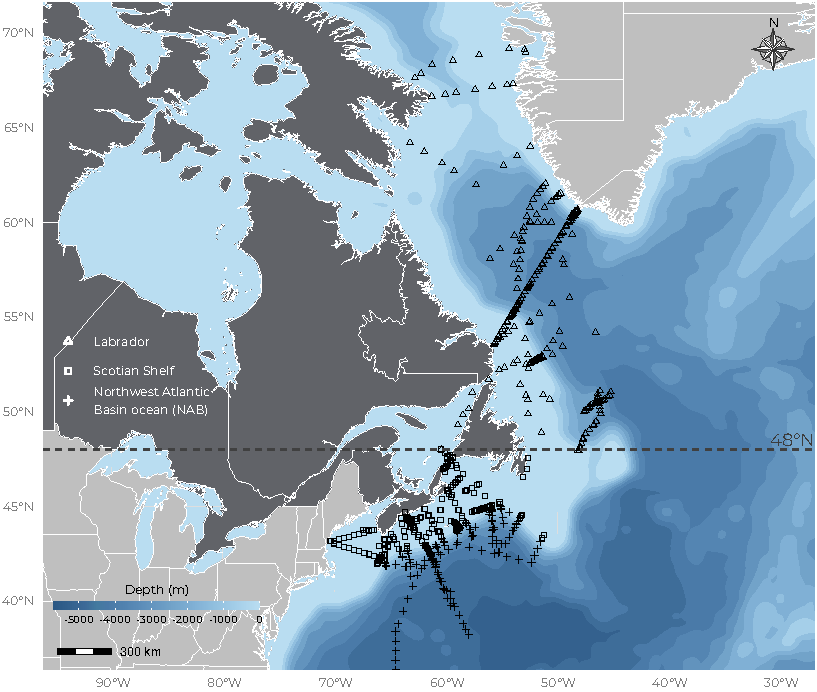
\includegraphics[]{../../../graphs/fig01.pdf}
    \end{center}
    \caption{This is a figure with sub figures, \textbf{(A)} is one logo, \textbf{(B)} is a different logo.}\label{fig:1}
\end{figure}

\begin{figure}[h!]
    \begin{center}
        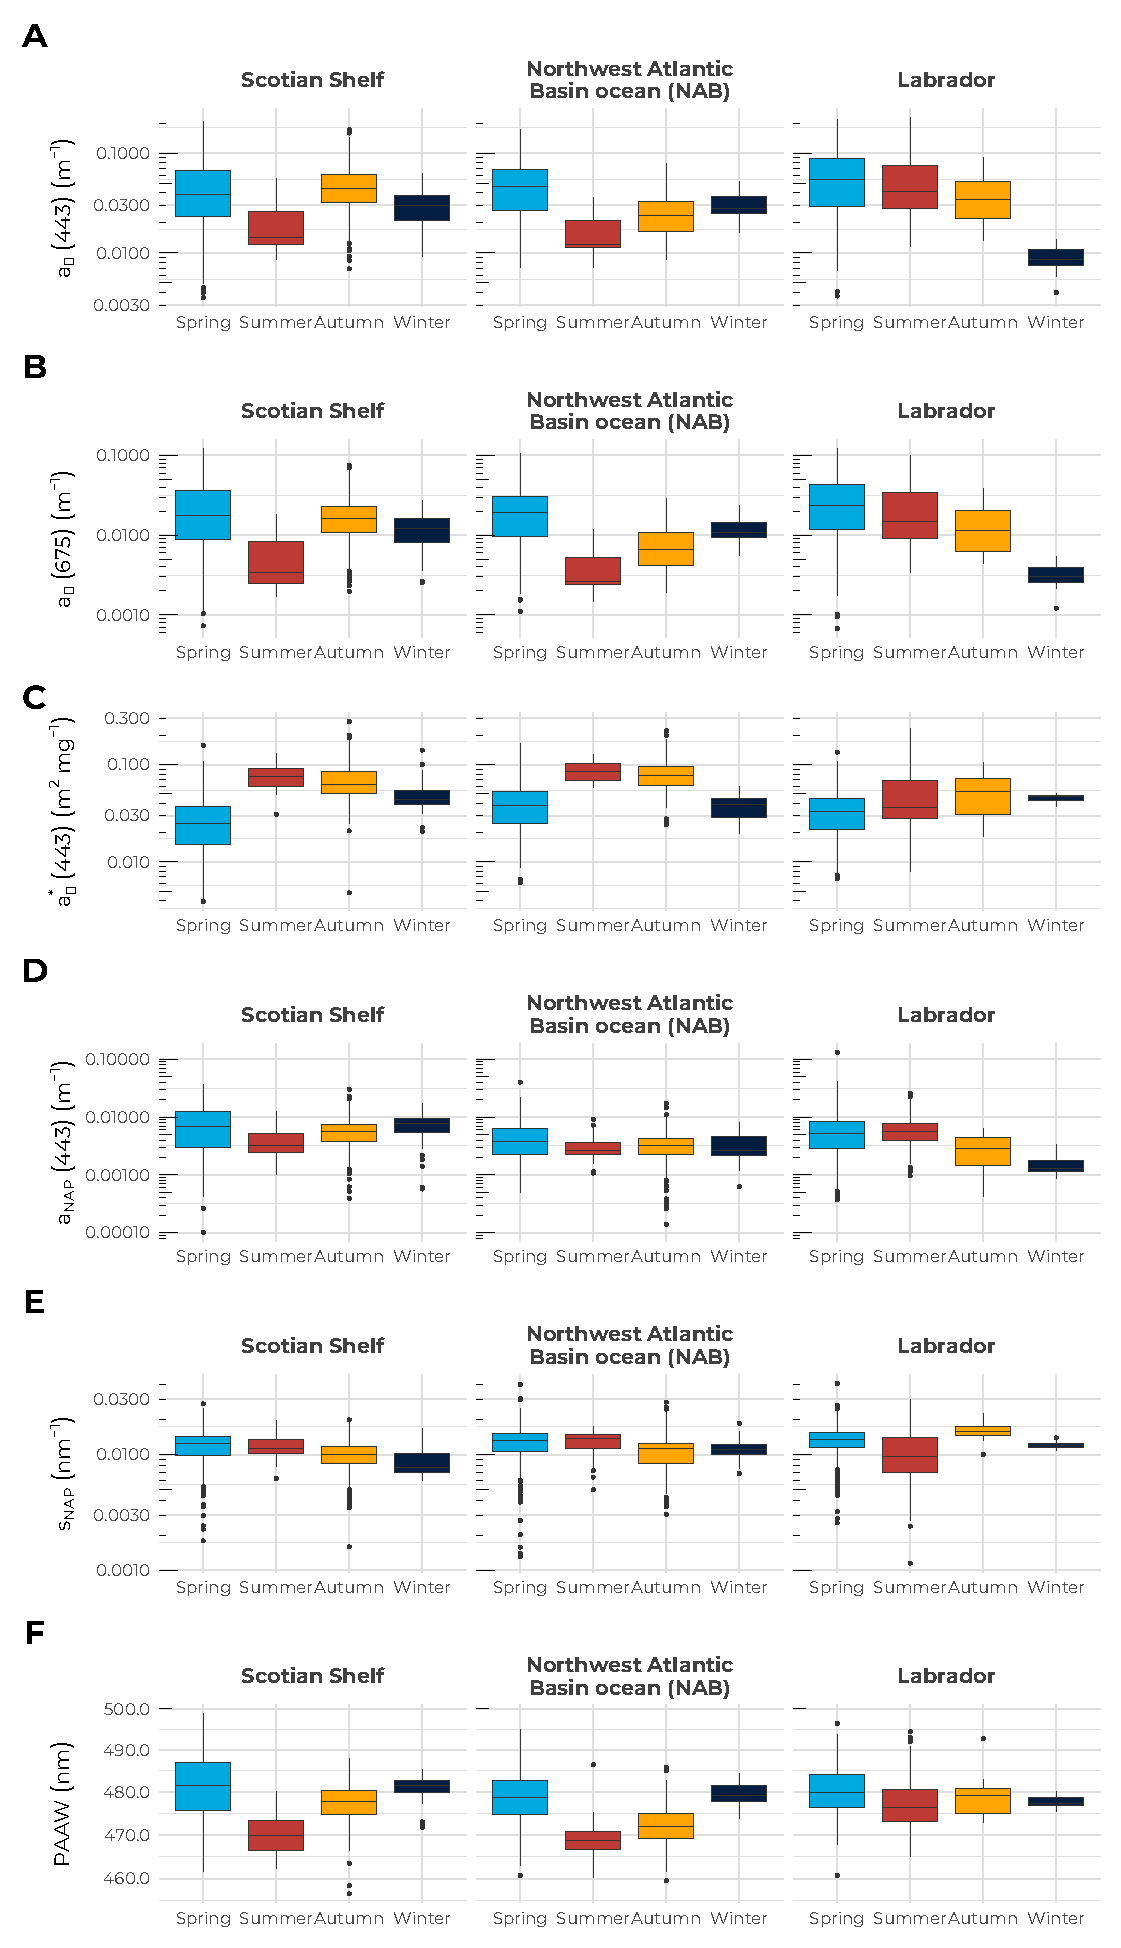
\includegraphics[]{../../../graphs/fig02.pdf}
    \end{center}
    \caption{This is a figure with sub figures, \textbf{(A)} is one logo, \textbf{(B)} is a different logo.}\label{fig:2}
\end{figure}


\begin{figure}[h!]
    \begin{center}
        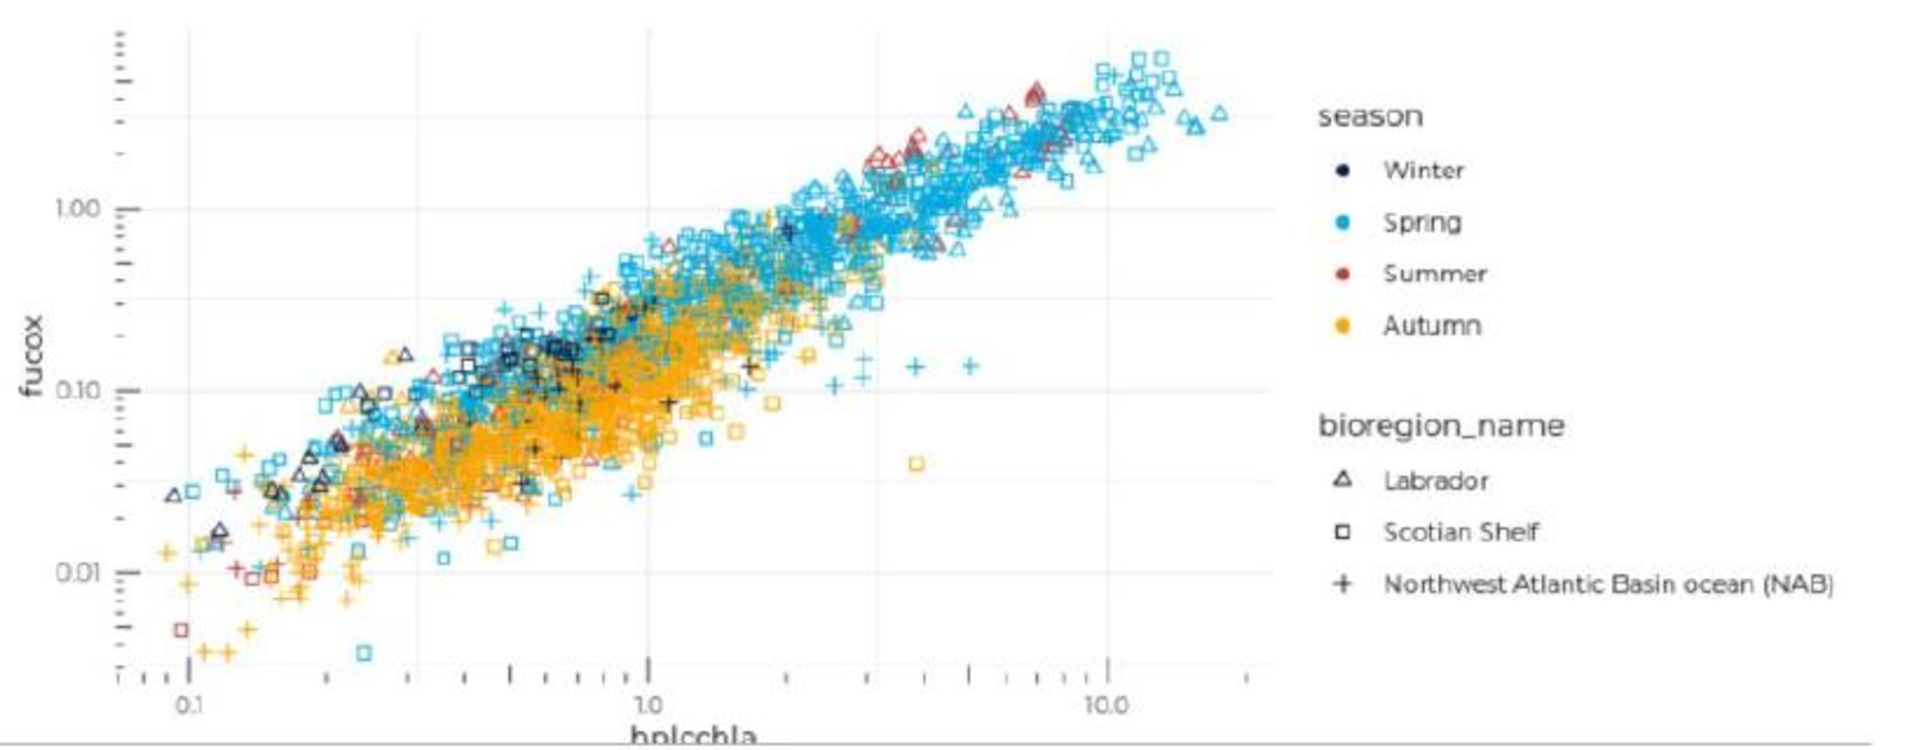
\includegraphics[]{../../../graphs/fig03.pdf}
    \end{center}
    \caption{This is a figure with sub figures, \textbf{(A)} is one logo, \textbf{(B)} is a different logo.}\label{fig:3}
\end{figure}


\begin{figure}[h!]
    \begin{center}
        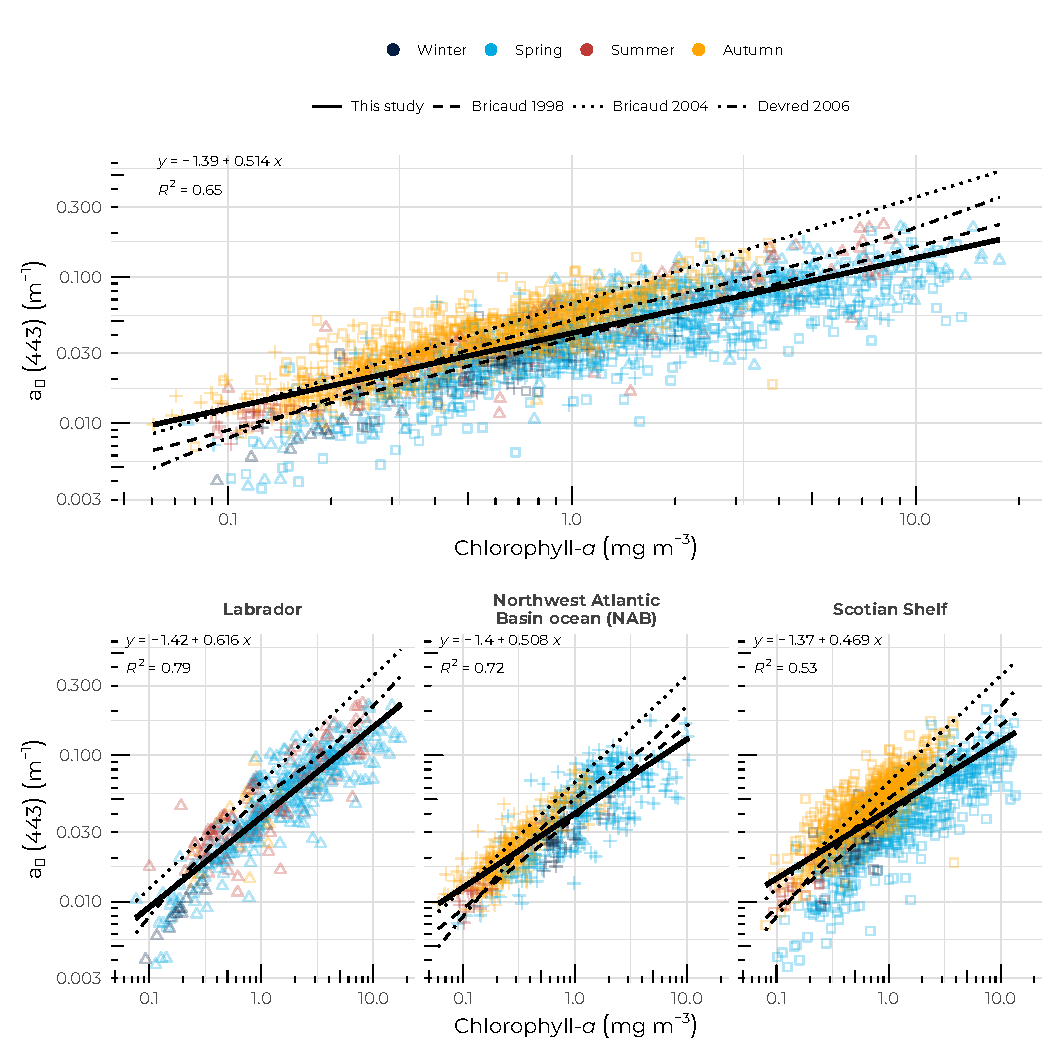
\includegraphics[]{../../../graphs/fig04.pdf}
    \end{center}
    \caption{This is a figure with sub figures, \textbf{(A)} is one logo, \textbf{(B)} is a different logo.}\label{fig:4}
\end{figure}


\begin{figure}[h!]
    \begin{center}
        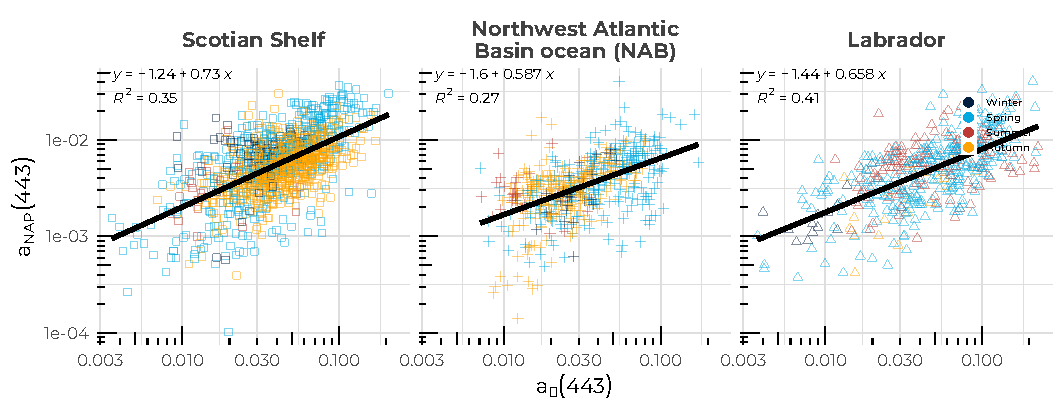
\includegraphics[]{../../../graphs/fig05.pdf}
    \end{center}
    \caption{This is a figure with sub figures, \textbf{(A)} is one logo, \textbf{(B)} is a different logo.}\label{fig:5}
\end{figure}


\begin{figure}[h!]
    \begin{center}
        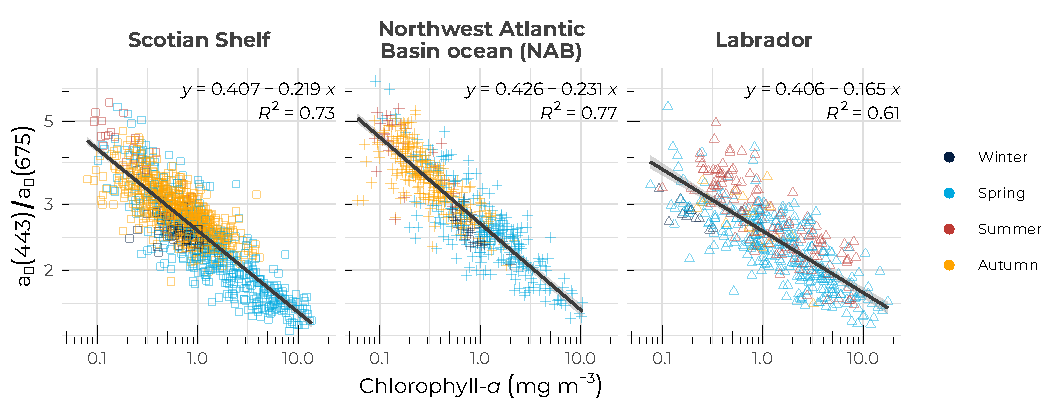
\includegraphics[]{../../../graphs/fig06.pdf}
    \end{center}
    \caption{This is a figure with sub figures, \textbf{(A)} is one logo, \textbf{(B)} is a different logo.}\label{fig:6}
\end{figure}


\begin{figure}[h!]
    \begin{center}
        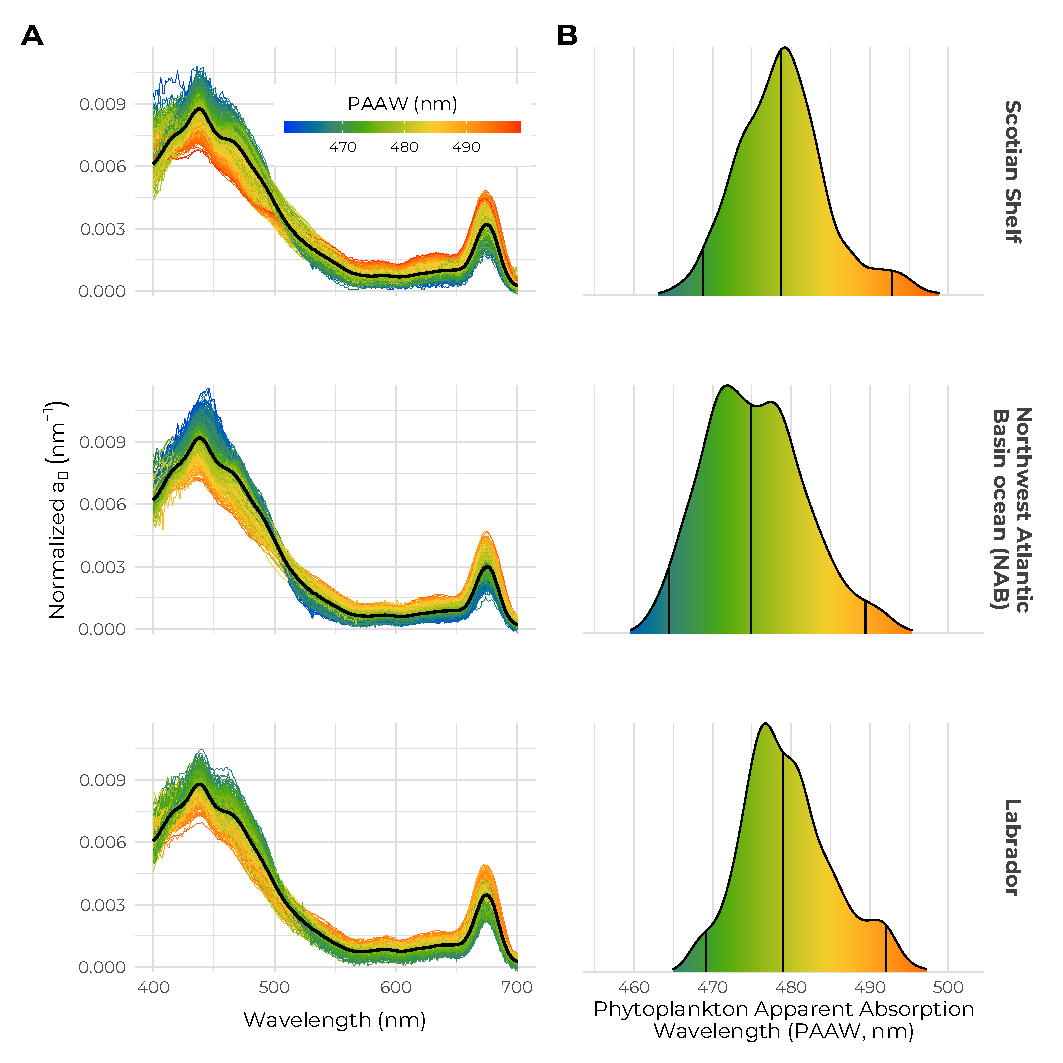
\includegraphics[]{../../../graphs/fig07.pdf}
    \end{center}
    \caption{This is a figure with sub figures, \textbf{(A)} is one logo, \textbf{(B)} is a different logo.}\label{fig:7}
\end{figure}


\begin{figure}[h!]
    \begin{center}
        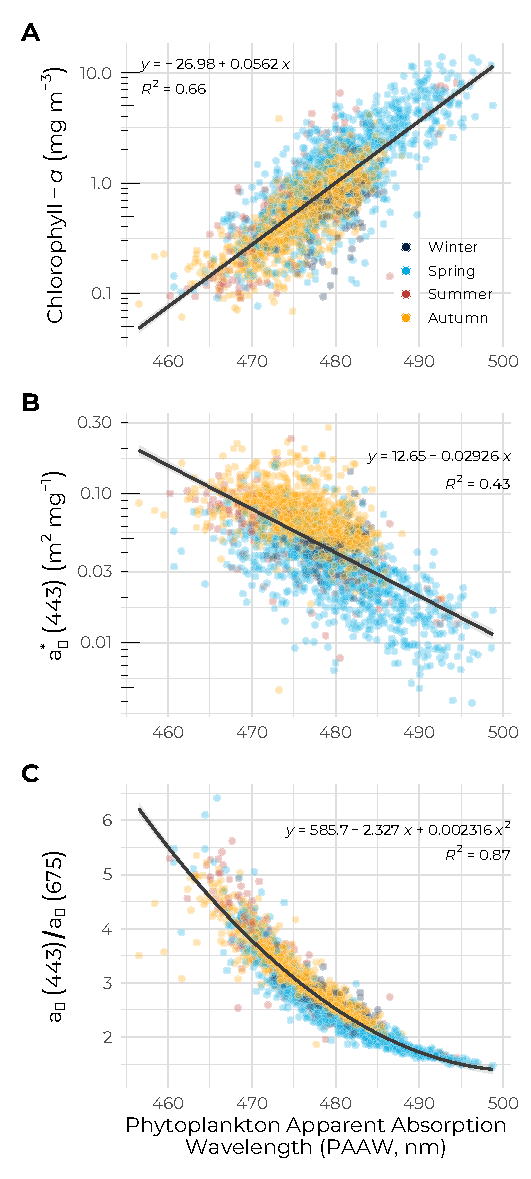
\includegraphics[]{../../../graphs/fig08.pdf}
    \end{center}
    \caption{This is a figure with sub figures, \textbf{(A)} is one logo, \textbf{(B)} is a different logo.}\label{fig:8}
\end{figure}


\begin{figure}[h!]
    \begin{center}
        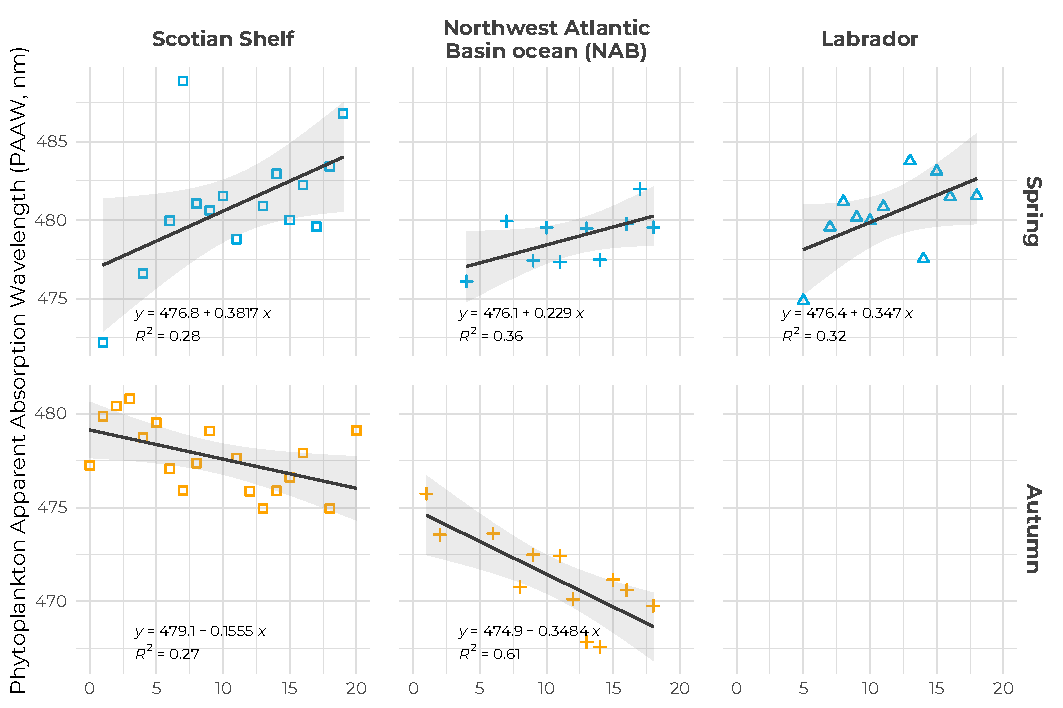
\includegraphics[]{../../../graphs/fig09.pdf}
    \end{center}
    \caption{This is a figure with sub figures, \textbf{(A)} is one logo, \textbf{(B)} is a different logo.}\label{fig:9}
\end{figure}


\begin{figure}[h!]
    \begin{center}
        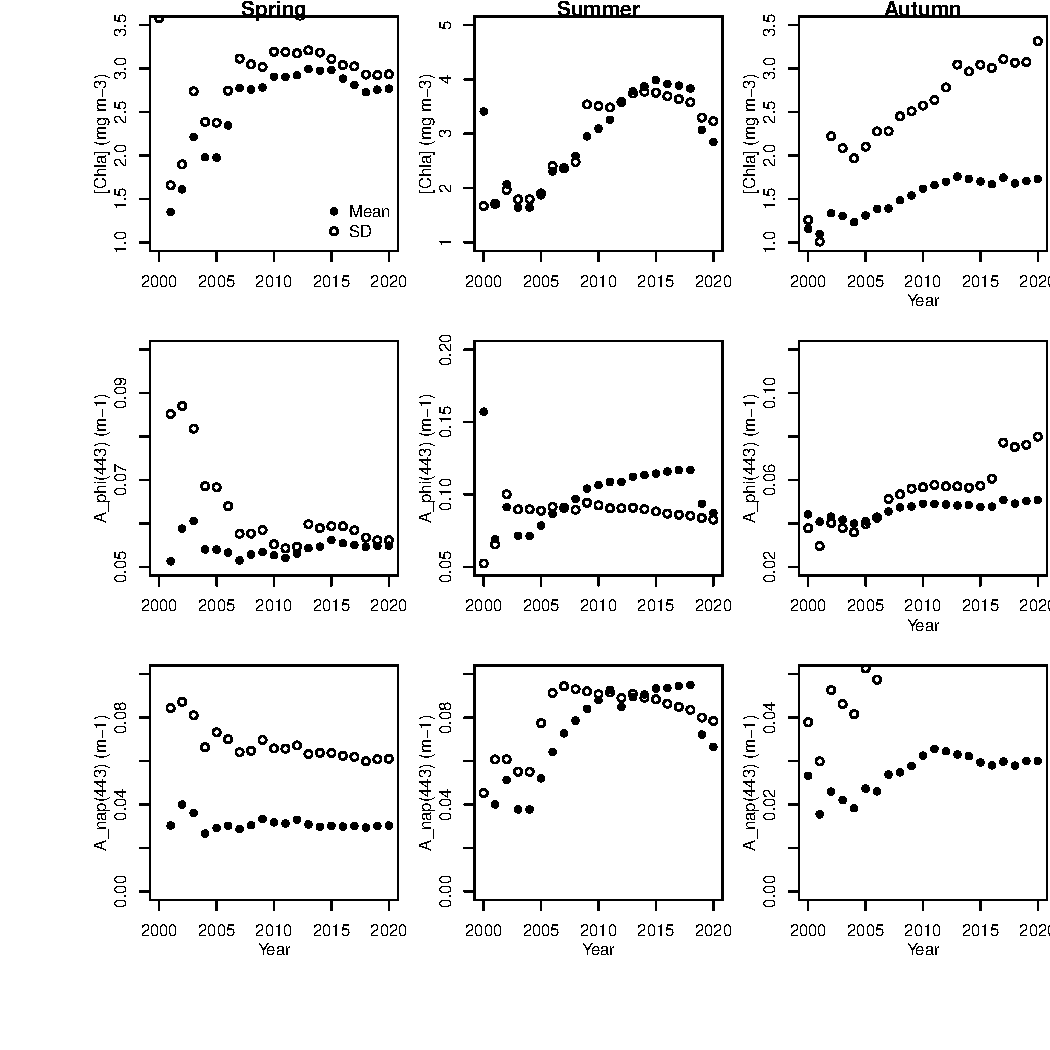
\includegraphics[]{../../../graphs/fig10.pdf}
    \end{center}
    \caption{This is a figure with sub figures, \textbf{(A)} is one logo, \textbf{(B)} is a different logo.}\label{fig:10}
\end{figure}


%%% If you are submitting a figure with subfigures please combine these into one image file with part labels integrated.
%%% If you don't add the figures in the LaTeX files, please upload them when submitting the article.
%%% Frontiers will add the figures at the end of the provisional pdf automatically
%%% The use of LaTeX coding to draw Diagrams/Figures/Structures should be avoided. They should be external callouts including graphics.

\end{document}
